\documentclass[a4paper,10pt]{article}
\usepackage[margin=1in]{geometry}
\usepackage{polski}
\usepackage[T1]{fontenc}
\usepackage[utf8]{inputenc}
\usepackage[unicode]{hyperref}
\usepackage{amssymb}
\usepackage{xifthen}
\usepackage[fleqn]{amsmath}
\usepackage{todonotes}
\usepackage{graphicx}
\usepackage{float}
\usepackage{fullpage}
\usepackage{epstopdf}
\usepackage{multirow}
\usepackage{subfig}
\usepackage{booktabs}
\usepackage[europeanresistors,americaninductors]{circuitikz}
\usetikzlibrary{patterns}
\newcommand{\withtodo}{0}

\def\arraystretch{1.2}

\begin{document}

\begin{table}
  \centering
  \def\arraystretch{1.5}
    \begin{tabular}{|c|c|c|c|c|} \hline
    \multicolumn{5}{|c|}{Wstęp do Fizyki Ciała Stałego}\\
		\multicolumn{5}{|c|}{Zadanie Projektowe} \\\hline
    Imię i nazwisko	&	nr albumu	&	grupa	&	data oddania	&	nr zestawu: 1	\\\hline
				Paulina			&		284494	&		R3	&								&	nr zadan:  \\
				Marikin			&						&				&								&	1,3,5 \\\hline
  \end{tabular}
\end{table}


\section{Zadanie 1: Analiza Termiczna}

\begin{figure}[H]
	\centering
		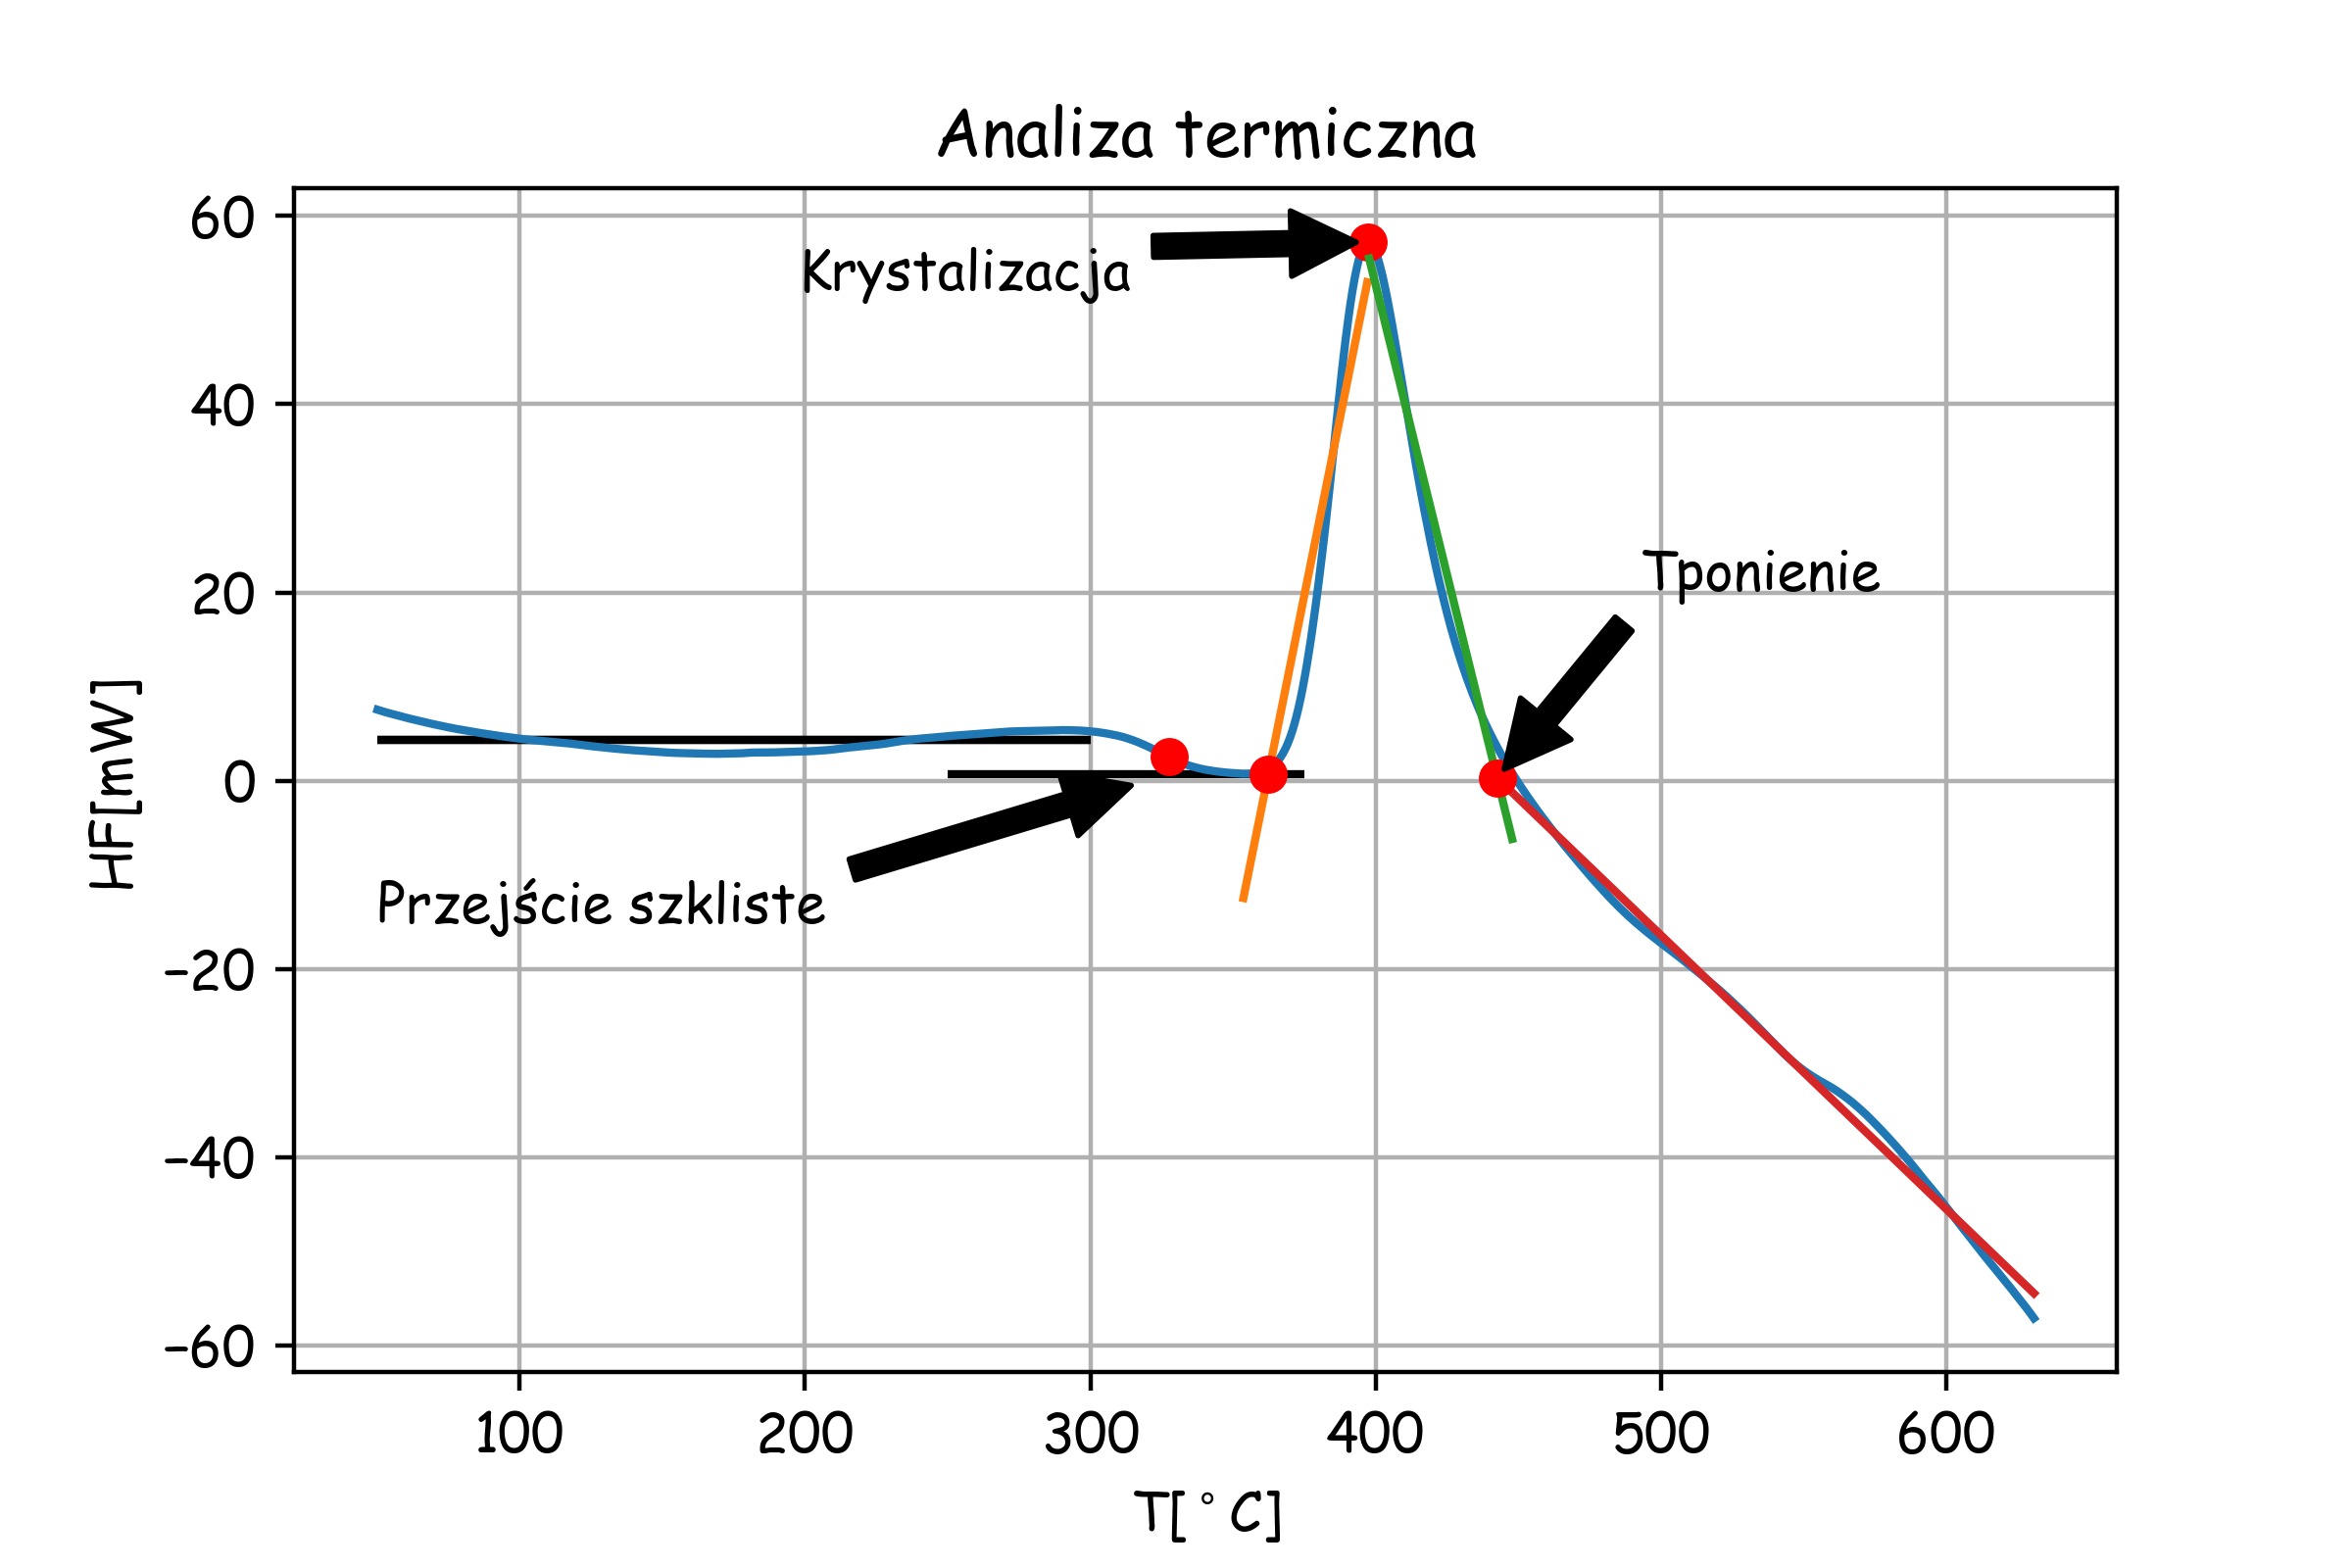
\includegraphics[width=\textwidth]{../Analiza_termiczna.png}
\end{figure}

\subsection{Przejście szkliste}
Temperatura: 327.571$^\circ$C \\
Wyznaczanie:
\begin{itemize}
	\item Dopasowanie prostej poziomej do początkowej cześci wykresu przed rozpoczęciem przejścia (do około 300 $^\circ$C).
	\item Wyznaczenie HF dla maksymalnego spadku temperatury po przejściu.
	\item Wyliczenie średniej z powyższych wartości
	\item Znalezienie pomiaru o HF najbardziej zbliżonym do danej średniej
	\item Temperaturę w tym pomiarze uznano za temperaturę przejścia szklistego
\end{itemize}

\subsection{Krystalizacja}
Temperatura początku krystalizacji:


\subsection{Topnienie}

\section{Zadanie 3: Dyfraktometria Rentgenowska}


\section{Zadanie 5: Testy Baterii Li-Ion}

 

\end{document}
